\documentclass[letterpaper,11pt]{article}
\oddsidemargin -1.0cm \textwidth 17.5cm

\usepackage[utf8]{inputenc}
\usepackage[activeacute,spanish, es-lcroman]{babel}
\decimalpoint
\usepackage{amsfonts,setspace}
\usepackage{amsmath}
\usepackage{amssymb, amsmath, amsthm}
\usepackage{comment}
\usepackage{float}
\usepackage{amssymb}
\usepackage{dsfont}
\usepackage{anysize}
\usepackage{multicol}
\usepackage{enumerate}
\usepackage{graphicx}
\usepackage[left=1.5cm,top=2cm,right=1.5cm, bottom=1.7cm]{geometry}
\setlength\headheight{1.5em} 
\usepackage{fancyhdr}
\usepackage{multicol}
\usepackage{hyperref}
\usepackage{wrapfig}
\usepackage{subcaption}
\usepackage{siunitx}
\usepackage{cancel}
\usepackage{mdwlist}
\usepackage{svg}
\pagestyle{fancy}
\fancyhf{}
\renewcommand{\labelenumi}{\normalsize\bfseries P\arabic{enumi}.}
\renewcommand{\labelenumii}{\normalsize\bfseries (\alph{enumii})}
\renewcommand{\labelenumiii}{\normalsize\bfseries \roman{enumiii})}


\begin{document}

\fancyhead[L]{\itshape{Facultad de Ciencias F\'isicas y Matem\'aticas}}
\fancyhead[R]{\itshape{Universidad de Chile}}

\begin{minipage}{11.5cm}
    \begin{flushleft}
        \hspace*{-0.6cm}\textbf{FI1000-1 Introducción a la Física Clásica}\\
        \hspace*{-0.6cm}\textbf{Profesor:} Ignacio Bordeu\\
        \hspace*{-0.6cm}\textbf{Auxiliares:} Alejandro Cartes \& Simón Yáñez\\
        \hspace*{-0.6cm}\textbf{Ayudante:} Javier Cubillos\\
    \end{flushleft}
\end{minipage}

\begin{picture}(2,3)
    \put(366, 10){
\includegraphics[scale=0.9]{2020-1/Imágenes/logo/dfi-fcfm.pdf}}
\end{picture}

\begin{center}
	\LARGE\textbf{Trabajo Dirigido \#1}\\
	\Large{Cinemática 1D y 2D}
\end{center}

\vspace{-1cm}
\begin{enumerate}\setlength{\itemsep}{0.4cm}

\rfoot[]{pág. \thepage}

\item[]

\item Dos autos (A y B) avanzan juntos por una calle, ambos con velocidad constante $v$. Cuando ambos autos están a distancia $L$ de un cruce se prende la luz amarilla del semáforo. El auto $A$ empieza a frenar con aceleración constante a modo de detenerse justo en el cruce. En tanto, el auto $B$ mantiene su velocidad. Transcurrido un tiempo $t_1$ desde que la luz cambió a amarilla, el semáforo cambia a rojo y entonces el auto $B$ empieza a frenar con aceleración constante para detenerse justo en el cruce (el auto $A$ sigue con aceleración que ya traía). Ambos autos se detienen exactamente en el mismo lugar.

\begin{enumerate}
    \item Muestre que es imposible que se detengan al mismo tiempo
    
    \item Grafique la posición y la velocidad de ambos autos en función del tiempo
\end{enumerate}

\item Desde la azotea de un edificio de altura $H$ se lanza una pelota con una velocidad inicial $v$ en una dirección $\theta$ con respecto a la vertical. A una distancia horizontal $D$ del edifico se encuentra otro edificio de altura $h$ ($h < H$) y longitud $L$. Determine el rango de valores que puede tener la rapidez para que la pelota no caiga fuera de la azotea del segundo edificio.

\begin{figure}[H]
    \centering
    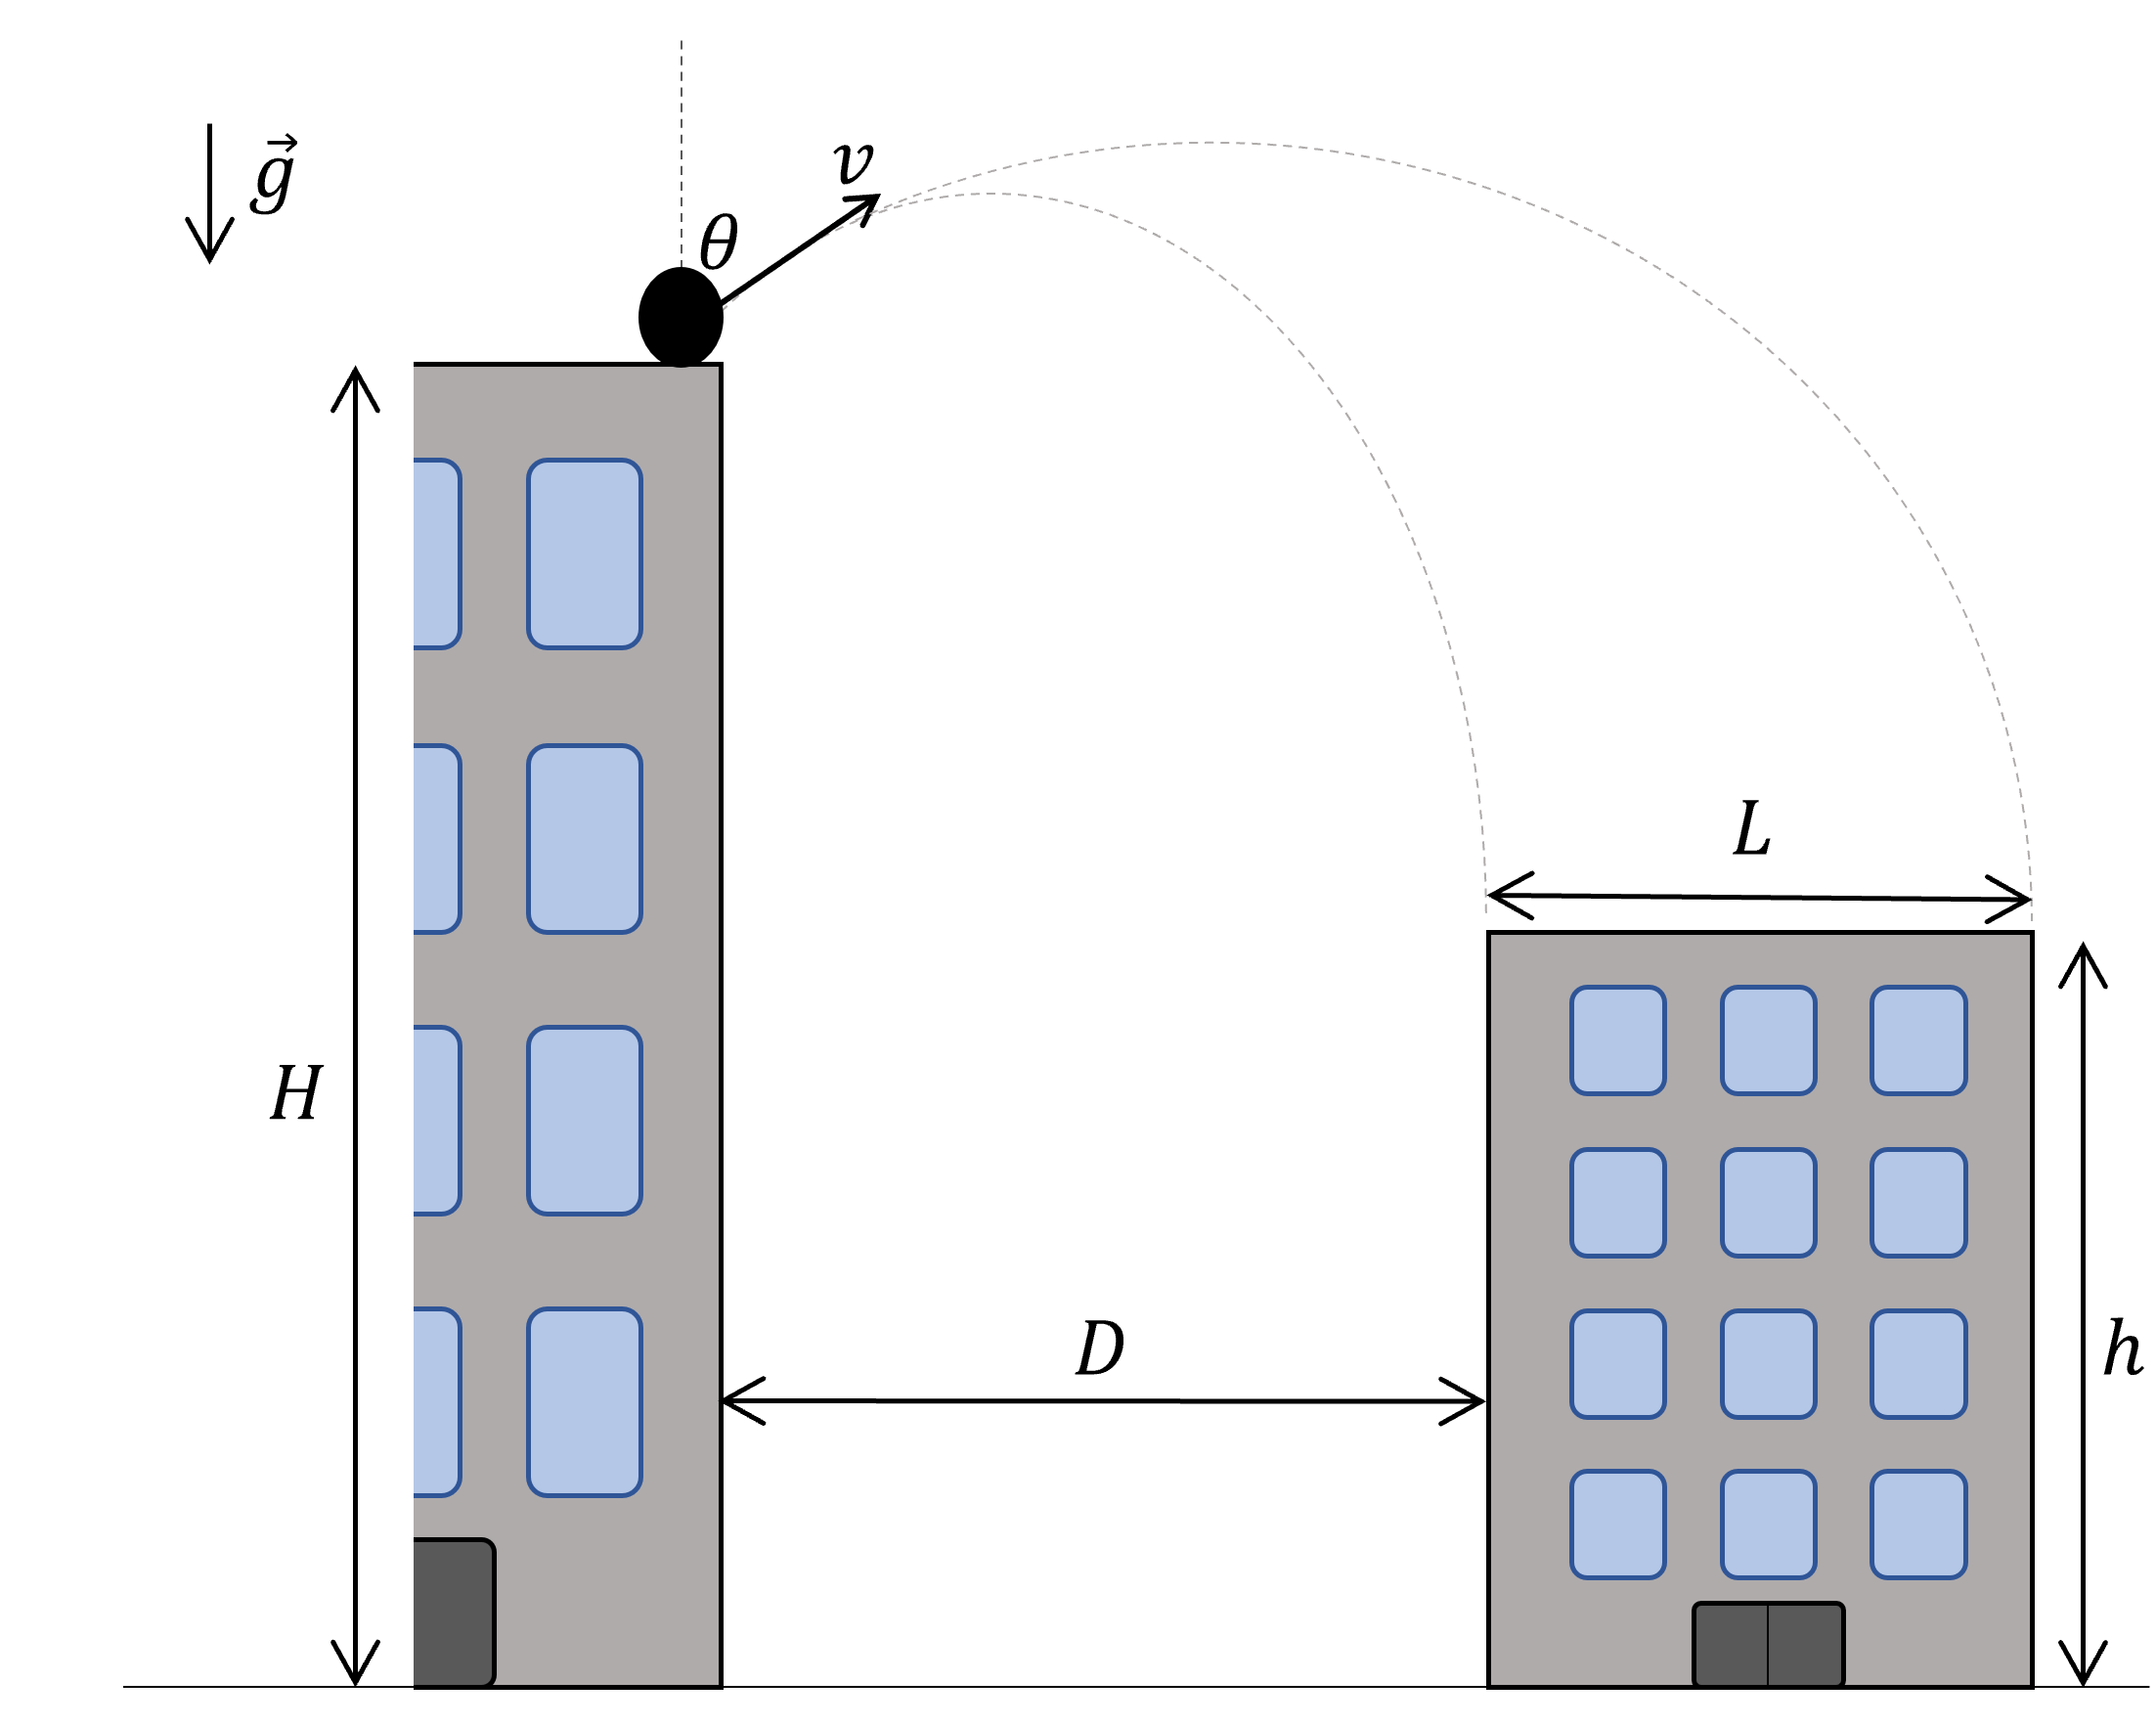
\includegraphics[width=0.4\linewidth]{2023-1/img/TD 1/edificios.png}
\end{figure}

\item 
\begin{multicols}{2}
Como se muestra en la Figura, se lanza un proyectil desde una ventana ubicada a una cierta altura. Dada una gran ventisca, existe aceleración horizontal $a_v$ que apunta en dirección al edificio, provocando que el proyectil se devuelva e ingrese a una ventana ubicada en un piso inferior. Si el proyectil se lanza con un ángulo $\alpha=45^{\circ}$ y rapidez $v_0$, determine:

\begin{enumerate}
    \item La distancia que separa a las ventanas por las cuales sale e ingresa el proyectil.
    
    \item La rapidez que tiene el proyectil al momento de ingresar por la ventana.
\end{enumerate}

\columnbreak

\begin{figure}[H]
    \centering
    \svgpath{../../2022-1/img/ejercicios}
    \includesvg[width=0.7\linewidth]{edificio.svg}
\end{figure}

\end{multicols}





% Para imágenes vectoriales -> el texto tiene que estar en LaTeX
% \begin{figure}[htbp]
%   \centering
%   \svgpath{../Imagenes/ejercicios}  -> .. irse pa'trás 
%   \includesvg{ej5.svg}
% \end{figure}

\end{enumerate}
\end{document}
